\begin{tabular}[t]{lp{\textSize}}
\hline
\hline

\raisebox{-0.84\totalheight}{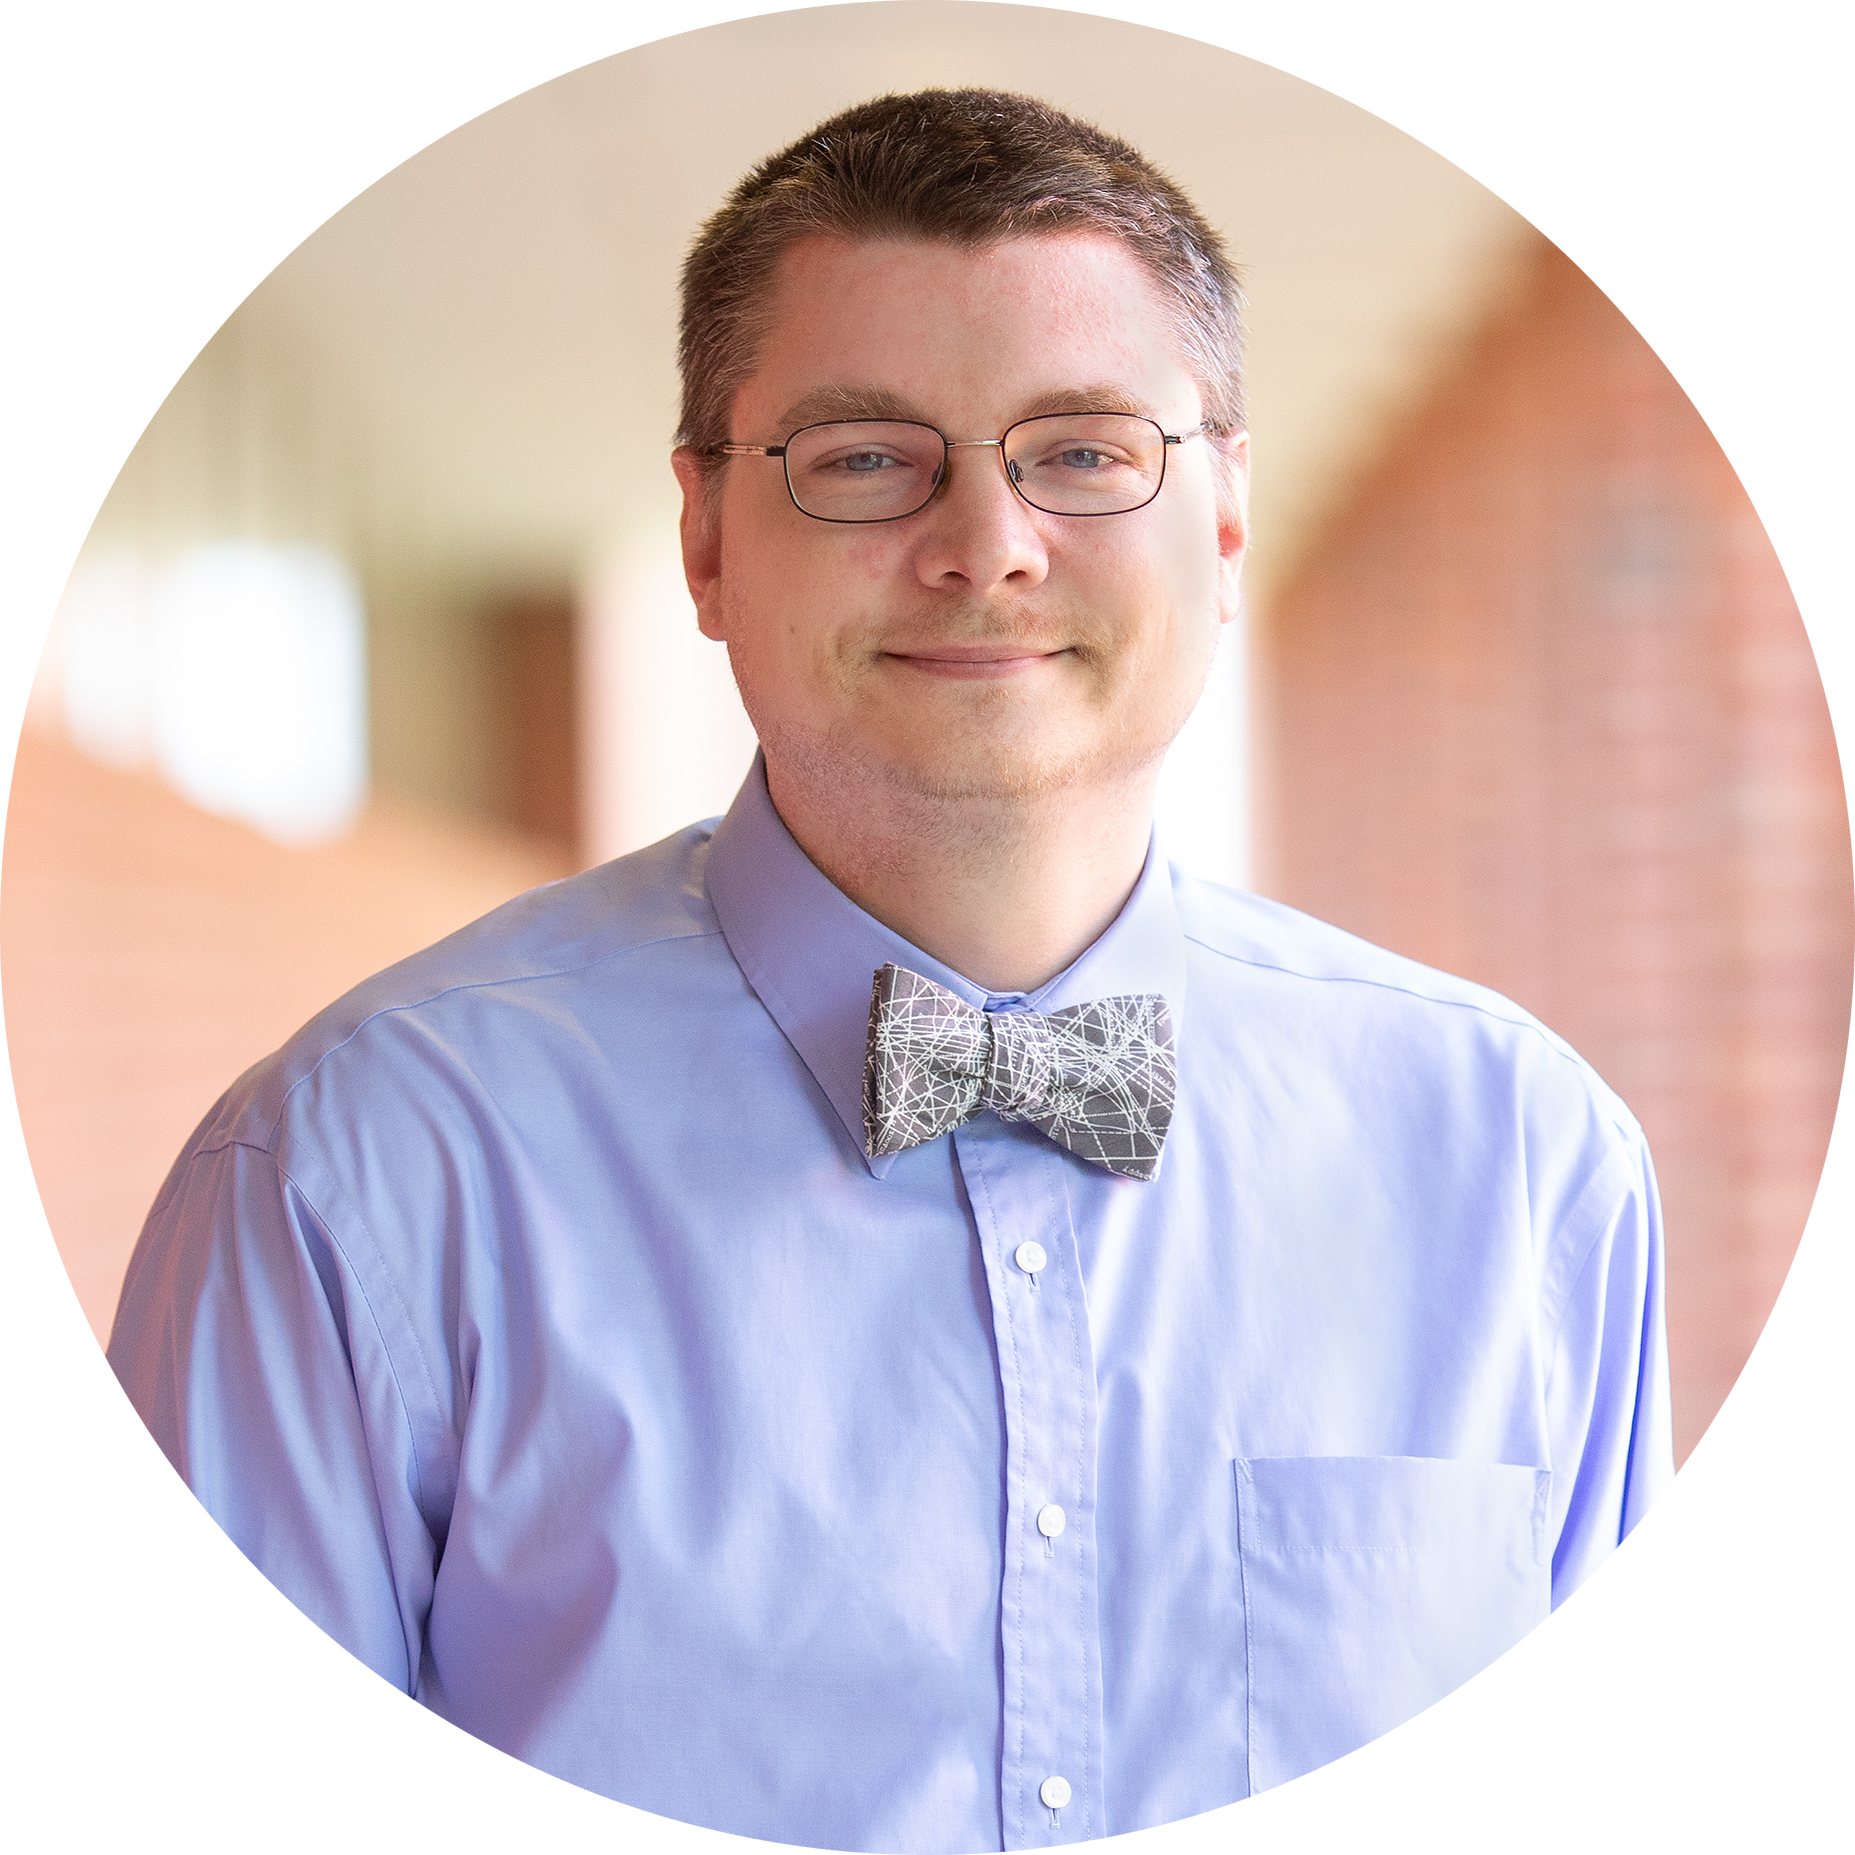
\includegraphics[width=\picSize]{images/people/alonzi.png}}
& 
\begin{tabular}[t]{p{\textSize}}
$\mathbf{Pete\:Alonzi}$ came to data science by way of the particle physics community. As a result, he has great interest in making data open and usable to broad audiences. He serves as a data scientist at the DSI and is the project manager for the Open Data Lab.
\end{tabular}
\\\hline

\raisebox{-0.84\totalheight}{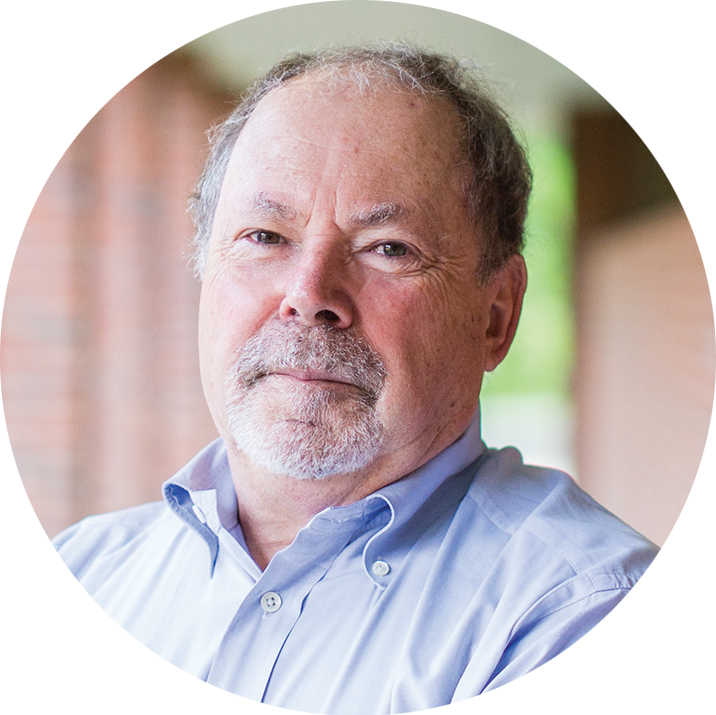
\includegraphics[width=\picSize]{images/people/bourne.png}}
 & 
 \begin{tabular}[t]{p{\textSize}}
$\mathbf{Phil\:Bourne}$, Stephenson Chair of Data Science and Director of the Data Science Institute. Before coming to serve at UVA Phil had been working for three years as the associate director for data science at the National Institutes of Health (NIH).
\end{tabular}
\\\hline

\raisebox{-0.84\totalheight}{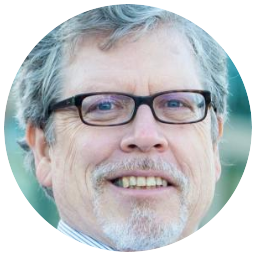
\includegraphics[width=\picSize]{images/people/clark.png}}
 & 
 \begin{tabular}[t]{p{\textSize}}
$\mathbf{Tim\:Clark}$, Ph.D., is a biomedical informatician and computer scientist with 28 years experience in academia, government, and industry.  He is an expert in data fusion and open science applications. He serves as an Associate Professor in the UVA School of Medicine \& the DSI. 
\end{tabular}
\\\hline

\raisebox{-0.84\totalheight}{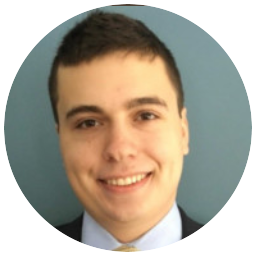
\includegraphics[width=\picSize]{images/people/levinson.png}}
 & 
 \begin{tabular}[t]{p{\textSize}}
$\mathbf{Max\:Levinson}$ is a Software Engineer and Cloud Developer in Public Health Services. When not building out REST apis for the NIH Data Commons Project, he can be found hacking on the Open Data Lab Project. Max is passionate about microservices development and anything Python. 
\end{tabular}
\\\hline

\raisebox{-0.84\totalheight}{\includegraphics[width=\picSize]{images/people/mietchen.png}}
 & 
 \begin{tabular}[t]{p{\textSize}}
$\mathbf{Daniel\:Mietchen}$ is a data scientist at the DSI. Trained as a biophysicist, he is interested in how research can be performed openly and collaboratively across traditional boundaries like disciplines, jurisdictions, economic sectors, languages, or professional versus volunteer participants.
\end{tabular}
\\\hline

\raisebox{-0.84\totalheight}{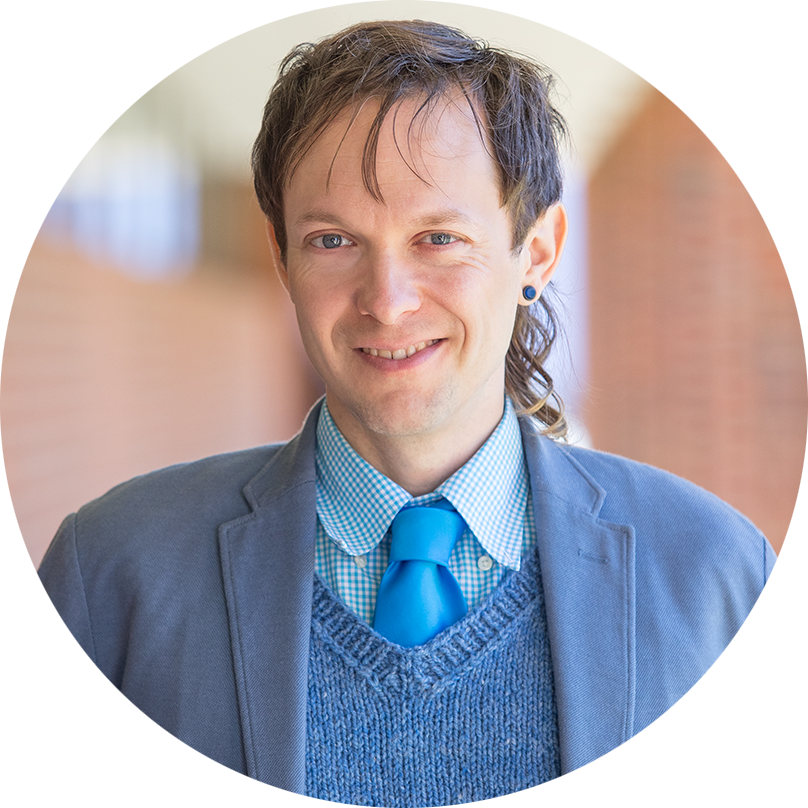
\includegraphics[width=\picSize]{images/people/rasberry.png}}
 & 
 \begin{tabular}[t]{p{\textSize}}
$\mathbf{Lane\:Rasberry}$ is a Wikimedia-in-residence.  His focus is using Wikimedia projects as a channel for publishing and distributing media from the DSI and UVA to an audience that engages with Wikimedia projects as an information resource and communication forum.
\end{tabular}
\\

\hline
\hline
\end{tabular}

% \smash{...} to override bounding
